\section{コンパにおける卓の振舞いについての基礎理論}
\rightline{文責:みそ汁}
\begin{multicols}{2}
\noindent{\uuline{\Large\textbf{1.はじめに}}}\\
\par
熊野寮では頻繁にコンパ(ないしは新歓)というイベントが開かれる。名前だけ列挙すれば、SC新歓、ティーパーティー新歓、ナス・サンマコンパ、全寮コンパ、お風呂入らない人コンパなどがある。コンパとは、大勢で食事をとりながら、寮生どうし(あるいは寮生と寮外生)で交流することだ。\footnote{あくまでコンパは他者と交流するためのものであって、食事をするためのものではないことに注意されたい。}。材料費などは寮の予算から出る。一言でコンパといっても様々なものがあり、食堂の机の上に料理を並べてつつくもの(ティーパーティー新歓など)、机をどけて畳を敷くもの(全寮コンパなど。今回分析対象としているのはこのような形のコンパである)、外でやるもの(ナス・サンマコンパなど)、など開催形態だけでも多くの種類がある。またお風呂入らない人コンパのように、料理が出ないものもある。
\par
コンパでは様々な属性を持つ人たちが同じ場所で食事をとるため、必然的に参加者の属性によっていくつかのグループに分かれる。このような小グループは「卓」と呼ばれる。例えば、A1ブロック\footnote{A棟1階のこと。熊野寮ではフロアごとに区分けして当番などを回している。区分けされた一つ一つをブロックと呼ぶ。各ブロックには1つ談話室があり、1つのコミュニティとなっている。}の人間だけが数人で集まって談笑している場合、そのグループはしばしばA1卓と呼ばれるし、3回生以上の人間だけが集まって談笑している場合、そのグループは老人卓と揶揄されることがある\footnote{熊野寮では4,5回生以上になって現役から引退(ブロックや部会、委員会での仕事を下回生に引き継ぐこと)した人々のことを老人と呼ぶことがある。そのような人たちがコンパの場で固まって1,2回生の知らない昔の寮生の話をしたりすることは、交流を生まないという観点から批判されることが多い。}。
\par
コンパの楽しみ方は様々なものがある。ただ人と交流するだけでも楽しいし、料理に舌鼓を打つのも一興だ。これらと同じぐらい、卓を観察するというのも楽しみ方の一つだと筆者は思う。卓がどのように生成し、その中でどのような動きがあって、どのように無くなっていくのか、ということを真面目に言語化している人は筆者の知る限りでは見たことがない。それゆえに、コンパにおける卓の振舞いには、新しい知見が眠っているのではないかと思うのである。
\par
以上に述べたことを背景として、本記事では卓を観察していく中で分かってきたことをいくつか論じる。一般に、寮内において「卓」という言葉は、コンパでできるグループのみならず、寮食を一緒に食べるグループ、食堂で勉強するグループなど、広く何らかの集団を指し示す言葉として用いられる。もちろんそうした意味での「卓」というものも興味深い考察対象ではあるのだが、一般論を述べる上では、コンパのような人の動きに物理的な制限がなく、他者との交流が制約なしになされる場が最も分かりやすい\footnote{例えば寮食を一緒に食べるグループは、机があって座る場所とグループの物理的な形が決められているという点や、一度席を決めたら移動することが困難である点で、人の動きに物理的な制限がある。また、寮食を複数人で食べる場合は仲の良い人同士で食べるというケースが多く、卓の振舞いを論じるにはやや特殊例となってしまう。}。そうした理由から、本記事ではコンパの卓に限って論じることにする。
\par
本記事では、卓がどのように生まれ(2.卓の生成)、どのように変化し(3.卓の拡大、分裂)、最終的にどうなるのか(4.卓の散逸、消滅)、ということについて概観する。さらに、こうした振舞いには卓の構成人数が大きな影響を与えているので、3章では卓の安定性と構成人数の関係性についても述べる。

\noindent{\uuline{\Large\textbf{2.卓の生成}}}\\
この章では卓ができあがる過程を描写するが、その前に卓とは何か、という問いに答えておかなければならない。本記事では、以下の3つの条件を満たしている集団を卓と呼ぶことにする。
\begin{itemize}
  \item 2人以上で構成されていること
  \item 互いにコミュニケーションをとっていること
  \item 構成員のどの2人も、互いに同じ集団に属していると認識しあっていること
\end{itemize}
つまり、卓とは大前提として2人以上の人の集まりでなければならず、そしてお互いに談笑する等のコミュニケーションをとっていなければならない\footnote{ここでは会話を聞いているだけの人も構成員とみなすことにする}。ただしコミュニケーションをとっていると言っても、例えば同じ鍋をつつきながらも会話をする際は身体の向きが正反対を向いている、というように、集団が誰もが分かる形で2つに分離していてはいけない、ということである。
\par
これをもとに、卓の生成過程は一言で「ぽつんと1人でご飯を食べている状態に、誰かしらが隣に座ってきて会話が始まること」と表現される。この話しかけてきた人は最初にいた人とどのような関係性なのかということについて考えてみると、多くの場合は最初にいた人の直接の知り合いであることが多い。新歓の場においては上回生が1人で食べている新入寮生に話しかけるというケースもしばしば目撃される。いずれにせよ、このようにして卓が生成する。
\par
小難しい理論だけ並べられても分かりにくいと思うので、1つ例を挙げることにする。本稿を通して、とあるコンパでの会話を例にとって説明する。なお、この会話はすべてフィクションである。
\par
\dotfill
\begin{itembox}[l]{登場人物}
  舞台はSC新歓\footnote{寮の新歓の中で一番最初に行われる新歓。食堂で大規模に開催される。コンパの代名詞のようなものである。}。新入寮生の自己紹介が終わり、コンパが再スタートしたタイミングである。
  
  \talker{佐藤}
  文学部1回生。D1ブロックに住んでいる。好奇心旺盛。
  
  \talker{鈴木}
  法学部2回生。\textgt{佐藤}と同部屋。

  \talker{高橋}
  文学部3回生。寮長をしているので新入寮生とたくさん話そうと息巻いている。

  \talker{田中}
  理学部2回生。\textgt{鈴木}とは同期なのでよく話す。

  \talker{伊藤}
  工学研究科M2。1回生の頃から寮生で、今やD1ブロックの長老となっている。この日も研究室にこもっていた。

  \talker{渡辺}
  総合人間学部1回生。コミュ力高め。
  
\end{itembox}
佐藤が料理を取り終え、畳に座る。一緒にいた鈴木が来るのを待っている。
\par
\talker{鈴木}
お待たせ。\textgt{〈卓の生成〉}

こうして鈴木が佐藤の隣に座ったときに、卓が生成した。
\par
\dotfill

\noindent{\uuline{\Large\textbf{3.卓の拡大、分裂}}}\\

\noindent{\uuline{\large\textbf{3.1.部分卓}}}\\
前章で述べたように卓が生成した後、その卓は人の動きにしたがって変化する。それは卓に人が加わる「卓の拡大」と、卓が二つに自然と分かれる「卓の分裂」の大きく二種類に分けられる。これからそれらの現象の様相を述べるわけだが、説明するには卓の中に卓のような構造を見出せると簡潔で都合がよい。そこで、主題に入る前に、部分卓という構造を導入しておく。
\par
卓の中に同じ属性を持っている2人以上のグループがある時、そのグループのことを部分卓という。このグループは2人以上で構成されており、同じ卓に属しているので互いにコミュニケーションをとっており、なおかつ構成員のどの2人も、互いに属性に共通するところがあり、かつ同じ卓に属していると認識している(互いに同じ集団に属していると認識している)ため、ある意味で卓の条件を満たしている。全ての卓はそれ自体の部分卓になっている。
\par
部分卓は様々なところで観測される。例えば、A1ブロック1回生が固まって話しているところに1回生とA1の住民が加わってできた卓は、A1卓と1回生卓を部分卓として持つことになる。

\noindent{\uuline{\large\textbf{3.2.卓の拡大}}}\\
人が一人加わって卓が出来上がると、たいていの場合、またもう一人話に加わってくる。そして3人の卓になったのちに、また再び一人話に加わり、4人の卓ができる。このように卓に新しく人が加わっていくことを「卓の拡大」と呼ぶことにする。また、第三者が卓に加わることを「参入する」と呼ぶ。この過程には、卓の構成人数や第三者の参入しやすさなどが大きな影響を与えている。順にみていこう。
\par
まず、前章で卓が生成したのちに、卓の構成人数が2人から3人に増えるときを考える(図\ref{fig:kakudai.flowchart}参照)。この時、もともといた2人が知り合いであれば、その2人の共通の知り合いや、少なくとも片方ととても親しい人間は、3人目として参入しやすい。反対にそうでない人間は参入しにくさを感じる。他方で2人が知り合いでない場合は、その卓は属性による排他性がなく、参入しやすさは誰でも同じである\footnote{誰でも同じというと少し分かりにくいかもしれない。人と話すのが得意な人と苦手な人では参入のしやすさが変わるのではないか、という指摘が予想されるからである。ただ、ここで言う参入しやすさというのはあくまで客観的な指標として捉えている。厳密に言えば、ここでは卓それぞれに”参入しやすさ”という客観的な指標が考えられると仮定し、その程度を議論しているのである。その人の持つ属性によって参入しやすさが変わるというのは、卓が持っている客観的な指標としての”参入しやすさ”が、特定の属性に向かって傾いている、という状態を意味している。それに加えて生じる個人差については、本記事では考慮していない。}。ここでの加わり方は、自分から入りにいく場合と2人のどちらかが引き入れる場合とに分かれる。多くの場合は前者で、後者の場合は3人目の人が2人のうち少なくとも片方と親しいときのみである。このときのように、卓の構成員がその人と親しい人や用事のある人に声をかけ、卓に参入させることを「引き込み」と呼ぶことにする。またこうした仕方で卓が拡大することを、「引き込みによる卓の拡大」ということにしよう。
\par
続いて卓の構成人数が3人から4人に増えるときを考える。この時、もともといた3人に共通した属性があれば、その人たちと同じ属性を持っている人は参入しやすく、持っていない人は参入しにくさを感じる。一方で3人に共通した属性がない場合、多くの卓では誰にとっても参入しやすさは変わらない。ただ、部分卓を持つ卓の場合は、部分卓の持つ属性を共通して持っている人は参入しやすくなる。ここでの4人目の加わり方は、2人の時と同様に自分から入る場合と引き込まれる場合とに分かれる。多くの場合には自分から入ることによって参入するが、引き込まれることも往々にしてある。ただ、引き込まれる側のハードルは、2人の場合よりも高くなることが多い。
\par
4人から5人に増える場合も同様に、4人に共通した属性があるならば、その属性を持っている人は参入しやすく、持っていない人は参入しにくさを感じる。一方で4人に共通した属性がない場合は、多くの卓では誰でも参入しにくさは同じであるが、部分卓を持つときは、部分卓の持つ属性と同じ属性を持っている人は参入しやすくなる。この時の拡大の仕方は、参入者が自分から入るケースと、引き入れによって拡大するケースとに分かれる。
\par
5人から6人に増える場合、6人から7人に増える場合等々、それ以降の拡大の仕方も似た様相を呈するが、5人以上の卓では、全員に共通した属性があることは珍しい。それゆえ、参入しやすさは基本的には人によって変わることはない。ただ、部分卓を持っていたり、引き込みが起きた場合はその限りではない。人数が多くなった分、参入という現象に与える部分卓の影響は他の要因よりも大きくなる。これは、知らない人が多い卓に参入する不安や恐怖が、知り合いが多い部分卓をよりどころにすることで解消されているからだと考えられる。また、卓の構成員からの引き入れも十分に発生し得る。
\begin{figure*}
  \centering
  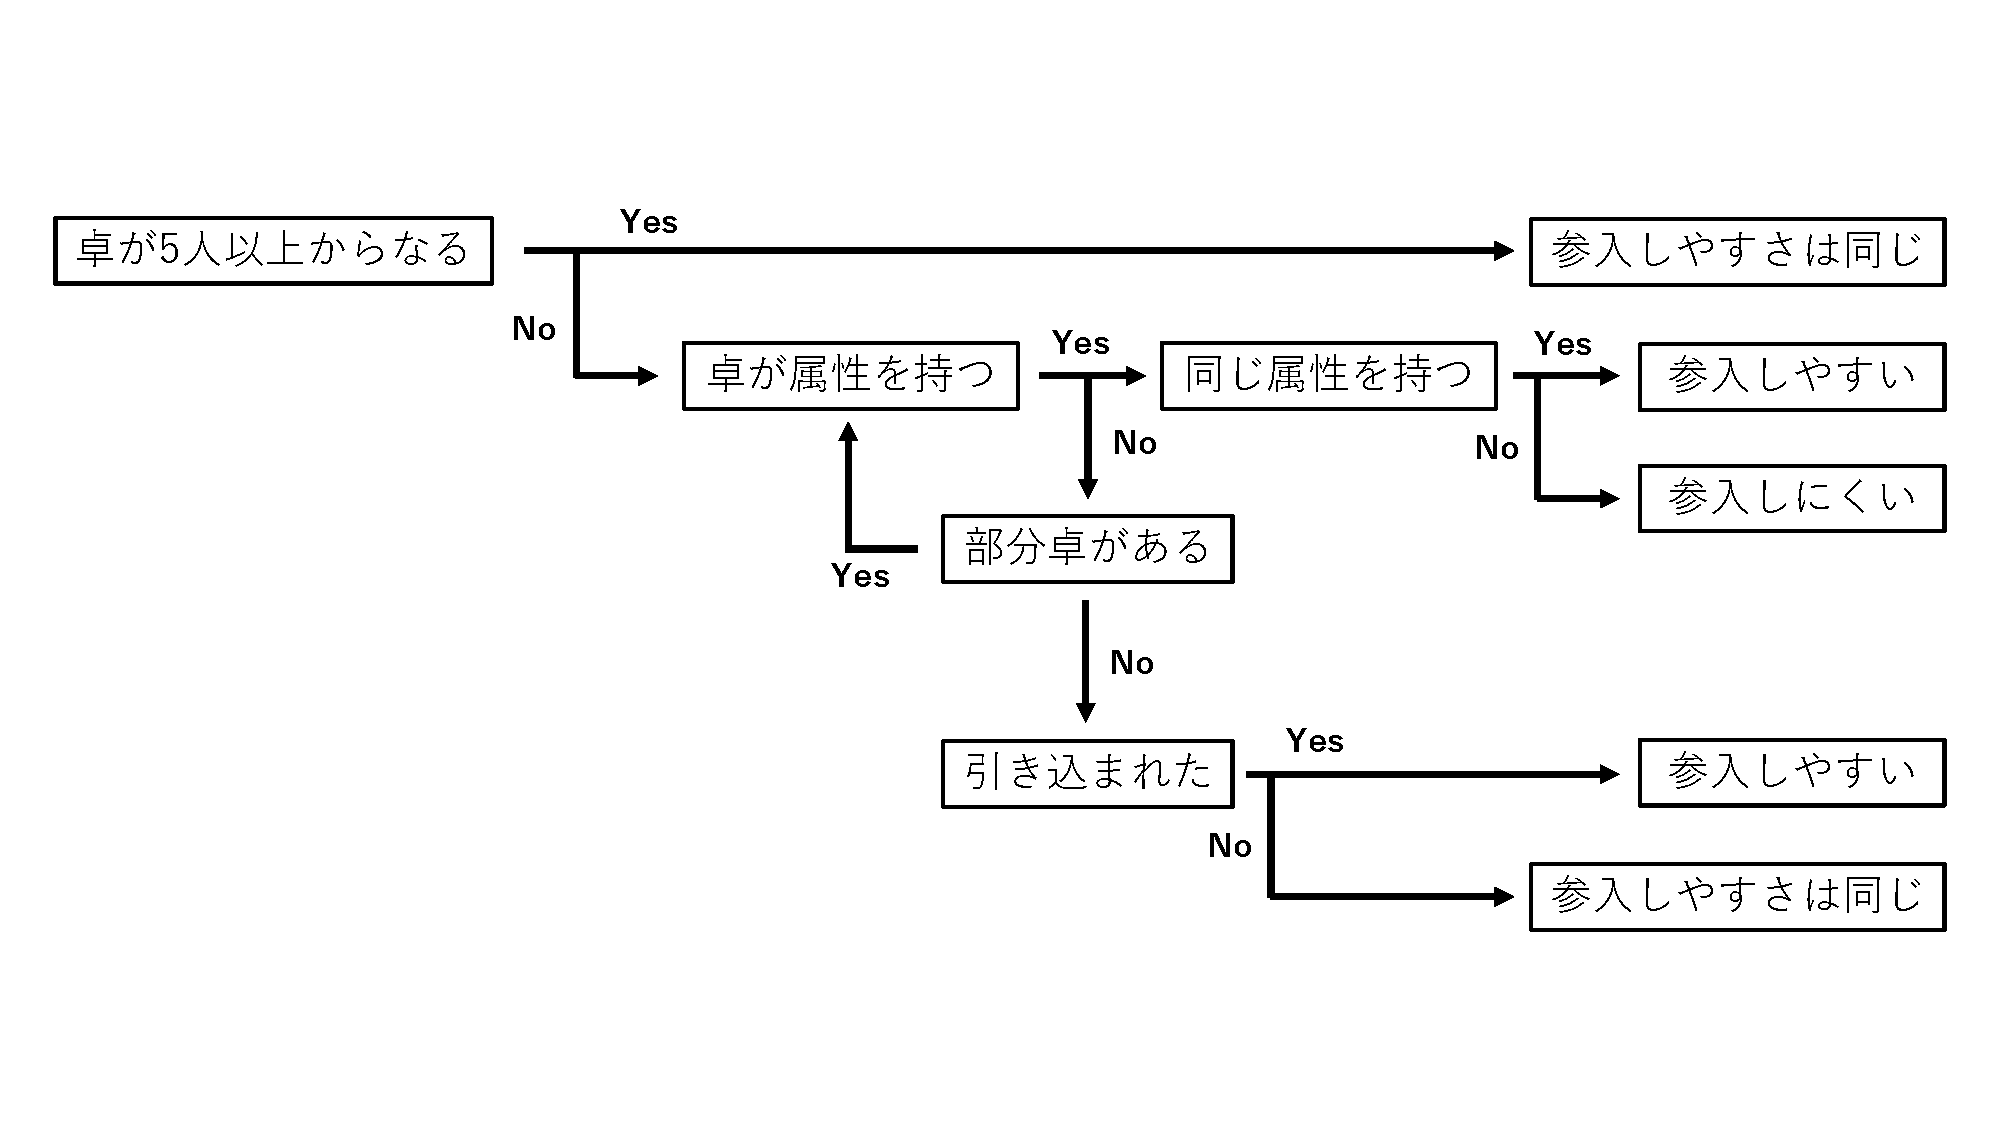
\includegraphics[height=6cm,width=12cm]{2025shinki/konpa_furumai/figures/takunokakudai_flowchart.pdf}
  \caption{拡大のフローチャート}
  \label{fig:kakudai.flowchart}
\end{figure*}
\par
前章で挙げた例では、次のように会話が進む。
\par
\dotfill
\par
\talker{鈴木}
自己紹介お疲れさま。

\talker{佐藤}
ありがとうございます。すごいですよね、めいも-------ん\footnote{SC新歓の自己紹介では、出身高校(または前の所属大学、予備校など)を言った後に参加者が「めいもーん」というコールをあげるという風習があった。自身の出自を明かすことを強制されるという側面に対する問題意識から、ここ数年でなくなってしまったが、筆者が入寮した時にはまだ残っていた。確かにノリについていける人とそうでない人で温度差はあったが、ああいった粗雑さの中に学生寮らしさを感じ取ったものだった。}って。出身校を名門だなんて言われたの初めてです。

\talker{鈴木}
ね。すごいよね。

高橋が加わる。佐藤の隣に座る。\textgt{〈卓の拡大\footnote{高橋が参入できたのは、恐らく高橋の立場やコミュ力の高さが原因だろう。}〉}
\par
\talker{高橋}
どーもー。

\talker{鈴木}
お疲れ様です。

\talker{高橋}
(佐藤に向かって)新入寮生の方ですか?

\talker{佐藤}
D101に住んでます、文学部1回生の佐藤です。

\talker{高橋}
佐藤さん。どうもD34に住んでる文学部3回の高橋です。

\talker{佐藤}
よろしくお願いします。

\talker{高橋}
寮で「佐藤さん」って意外と珍しいよね。

\talker{鈴木}
ですよね。

\talker{佐藤}
そうなんですか?

\talker{高橋}
そう。珍しい苗字は時々見かけるけど、この寮意外とメジャーな苗字がいなかったりするんだよね\footnote{これはその通りで、熊野寮ではメジャーな苗字は意外と見かけなかったりする。そこまで多くない苗字が意外と寮内ではメジャーな苗字だったりもする。}。

\talker{佐藤}
へぇ~。

田中がそばを通る。
\par
\talker{鈴木}
あ、田中だ。おーい。
\par
田中が加わる。鈴木と高橋の間に座る。\textgt{〈引き込みによる卓の拡大\footnote{田中が鈴木の隣に座ったのは、鈴木に引き込まれたからである。}〉}
\par
\talker{田中}
こんにちは~。

\talker{鈴木}
この子同部屋の1回生の子。

\talker{田中}
お~。(拍手)

\talker{佐藤}
D101の佐藤です。

\talker{田中}
田中と言いますぅ。

\talker{佐藤}
田中さんの学部はどちらですか?

\talker{田中}
理学部だよー。

\talker{佐藤}
理学部。へ~。

\talker{田中}
今年系登録できるか微妙だからやばい(笑)(ピース)

\talker{鈴木、高橋}
(笑い)

伊藤が加わる。佐藤と高橋の間に座る。\textgt{〈卓の拡大\footnote{なぜ鈴木の隣に座らなかったのか疑問に思った読者もいるかもしれない。しかし、もし伊藤が元寮長だとすれば、あるいは伊藤が新歓の場では積極的に1回生に話しかけに行くタイプであったとすればどうだろう。}〉}
\par
伊藤が加わった後の位置関係は図\ref{fig:example.2}のようになっている。ただし、三角形の向く方向はその人の身体や顔の向きを表している。
\begin{figure*}[htbp]
\begin{minipage}[b]{0.45\linewidth}
   \centering
  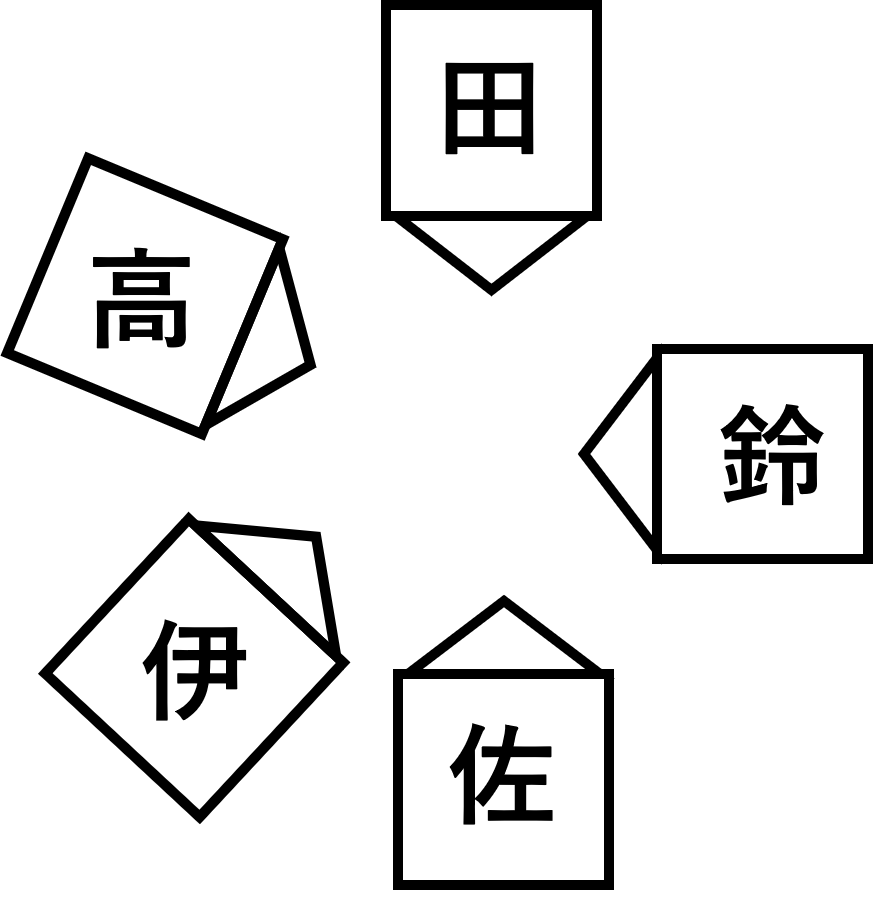
\includegraphics[height=4cm,width=4cm]{2025shinki/konpa_furumai/figures/taku.example_2.png}
  \caption{伊藤が加わった後の卓}
  \label{fig:example.2}
\end{minipage}
\begin{minipage}[b]{0.45\linewidth}
  \centering
  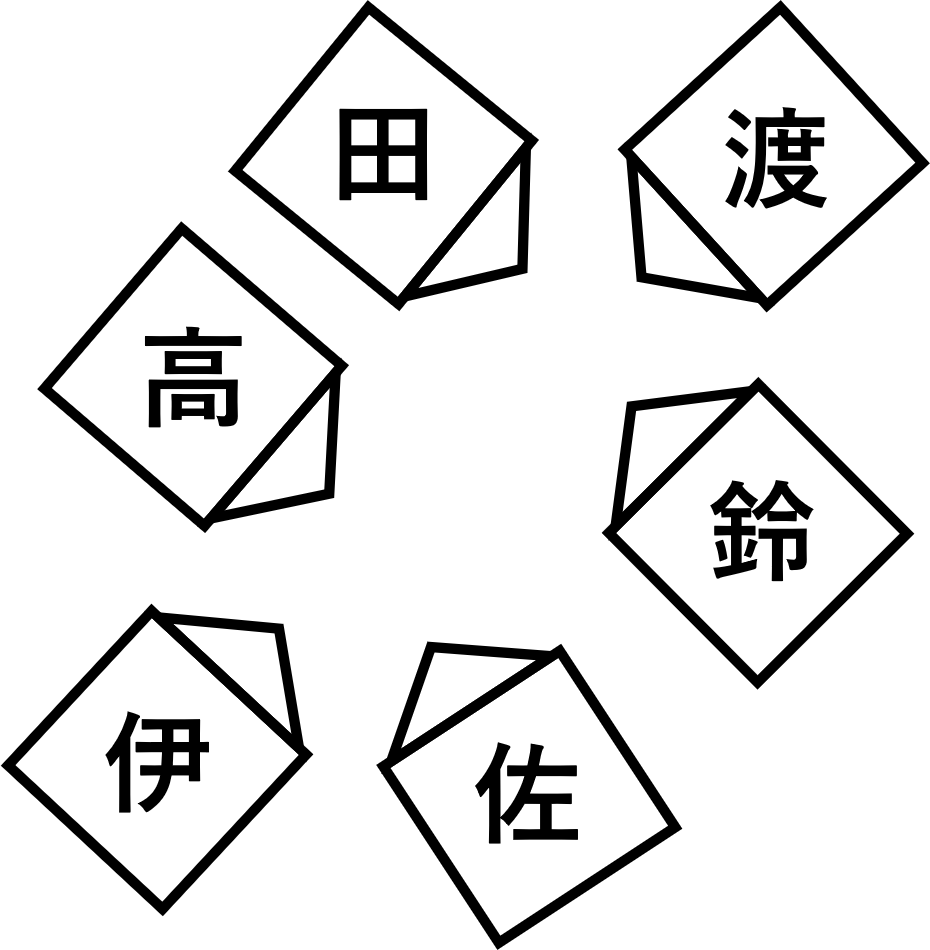
\includegraphics[height=4cm,width=4cm]{2025shinki/konpa_furumai/figures/taku.example_3.png}
  \caption{渡辺が加わった後の卓}
  \label{fig:example.3}
\end{minipage}
\end{figure*}
\par
\talker{伊藤}
お邪魔しま~す。

\talker{鈴木}
伊藤さん。うちのブロックの1回生の子です。

\talker{佐藤}
D101の佐藤です。

\talker{伊藤}
どうも工学研究科M2の伊藤です。来年退寮する老人です。学部はどこ?

\talker{佐藤}
文学部です。

\talker{伊藤}
へぇ~。どの分野やりたいとかあるの?

\talker{佐藤}
近世哲学とか興味あります。

\talker{伊藤}
カントとかヘーゲルとかのあたり?

\talker{佐藤}
あー、そうですそうです!

\talker{伊藤}
へ~。そこらへんは倫理で習っただけであんまり知らないけど面白そうだよね。熊野寮って哲学好きな人結構多いし。楽しめるんじゃない?

\talker{佐藤}
やっぱりそういう人多いんですか?

\talker{伊藤}
ごりっごりの哲学という感じではないけどそっち方面の話題が好きな人はやっぱり多いね。前に出てくる人とかごりごり寮自治してるよ、っていう人とかにそういう人が多いだけかもしれないけど。会議とか出てると「寮自治は何のためにやるのか」とか「寮祭はなぜやるのか」とかそういう話になることがしょっちゅうあるねー。

\talker{佐藤}
へー。面白そう。

\talker{伊藤}
お〜。これを面白いと思える人は結構寮生活向いてるよ。新歓とかたくさん行くと知り合いもたくさんできるし授業始まってからもすっごい楽しくなるから、自分の部屋とかにこもらずにどんどん談話室とか食堂とかに顔出すといいよ\footnote{文学部で、哲学好きで、なんとなく態度が前のめり。この卓の人間は皆、\textgt{佐藤}はこれから寮自治の中心に関わっていくに違いないと考えているだろう。ただ、登場人物たちは\textgt{佐藤}が好奇心旺盛であるという点を知らない。好奇心だけで動く人間は寮自治ではなく自治寮に興味があることが多い。自治活動に関わるきっかけの一つとして好奇心は重要だが、上回生になれば寮を維持・発展させるという責任感を持つことも求められる。}。
\par
\dotfill

\noindent{\uuline{\large\textbf{3.3.卓の分裂}}}\\
卓は人数が多くなると、違う話題を話す2つの卓に分かれることがある。これを「卓の分裂」と呼ぶことにする。分裂してできたひとつひとつのグループは、その内部で同一のグループに属しているという共通認識を持つことが多いので、それぞれが卓の条件を満たしている。
\par
分裂の仕方を一言で表現すると、同じ卓の中で違う会話の流れが生まれるということである。卓の振舞いで転機となるのは、複数人が同時に話始めることや、自分が話さない時間が長くなったりすることだ。複数人が同時に話し始めると、同じ卓の中で違う話を聞き始める人が生まれる。それぞれの話から再び会話が始まるので、違う会話をする2つのグループが生じ、それぞれ卓として振る舞うようになる。また、自分が話さない時間が長くなると、手持ち無沙汰になって隣の人と世間話をする人が出てくる。これによって複数人が同時に話始める状態が生まれ、上と同様にして卓が分裂する。さらに進むと、人の配置が変化して2つの輪ができる。そこまでくれば分裂したことは外から見ても明らかである。
\par
分裂のしやすさは、拡大といった他の要因を考えなければ卓の構成人数が多くなるほどしやすくなる。なぜなら、人数が多くなればその分自分が話さない時間が長くなったり、同時に複数人が話始めるタイミングが多くなるからだ。
\par
これまで述べた例でも卓の分裂を見てみる。
\par
\dotfill
\par
先ほど述べた例の最後の方では伊藤と佐藤の会話がメインであった。伊藤の話す時間が長くなったので、ここから卓が分裂していく。現在各登場人物の状況は以下のとおりである。
\begin{itembox}[l]{各登場人物の状況}
  \talker{佐藤}
  伊藤と話している。
  
  \talker{鈴木}
  佐藤がいい感じに会話に溶け込めてきたので、あとは気さくな伊藤に任せて他の参加者とも話そうかと思っている。
  
  \talker{高橋}
  できれば新入寮生と話したいので\textgt{佐藤}と\textgt{伊藤}の会話に参加しようと思っている。
  
  \talker{田中}
  手持ち無沙汰になっている。
  
  \talker{伊藤}
  佐藤と話している。
\end{itembox}
田中が鈴木に話しかけるところから卓の分裂が始まる。

\talker{田中}
鈴木は春休み何してたー?\textgt{〈卓の分裂〉}

\talker{鈴木}
何もしてない。談話室でごろごろしてたら2か月過ぎてた\footnote{あるある。談話室にいると何故か時間が溶けていく。}。

\talker{田中、鈴木}
(笑い)

\talker{鈴木}
田中は?

\talker{田中}
さすがにそろそろ頑張らないとやばいと思って、1回生の復習とかやろうとしてたら、なんか春休み終わってた~。

同時並行で進んでいる伊藤と佐藤の会話も見てみよう。
\par
(前項の会話の続きから)
\par
\talker{佐藤}
へ~。寮の新歓結構多いですよね。明日はD34?新歓がありますし。

\talker{高橋}
そう!明日D34新歓やるから来てね。

\talker{佐藤}
あ!確かに高橋さん?はD34ブロックでしたね。

\talker{伊藤}
めっちゃ食い気味(笑)。こっからブロック新歓って言って、各ブロックが主催する新歓が始まるんだけど、その1発目がD34の主催するD34新歓。ブロック新歓はブロックごとに特色があって面白いよ\footnote{筆者にとってブロック新歓巡りは春新歓の楽しみの一つである。新歓で提供される料理や、新歓内で行われるレクリエーションには、そのブロックの工夫やノリが垣間見えて面白い。1回生の時もブロック新歓は楽しみであったが、新歓を主催する側になると今度は料理の工夫やレクのアイデアを盗みたいと思うようになり、また楽しみが増えた。}。

\talker{佐藤}
へ~。楽しみです。
\par
\dotfill

\noindent{\uuline{\large\textbf{3.4.卓の安定性}}}\\
この章で述べた卓の拡大や分裂により、卓の安定性を考えることができる。まず、卓が安定しているとは、拡大も分裂もしにくい状態、すなわち卓の構成人数が変化しにくい状態のことであると定義する。本来卓の安定性には構成員の属性といった、様々な要因が影響していると考えられる。ただ、安定性の複雑な様相を論じることは本記事の趣旨から外れてしまうので、ここでは構成人数による安定性の変化について述べるにとどめる。
\par
まず拡大のしやすさに目を向ける。卓の構成人数が多くなりすぎると、物理的に参入できなくなるので卓は拡大しにくくなる。筆者の経験では、5人以上になると明確に拡大しにくくなる。これよりも人数が少ない場合を考えると、部分卓の属性が薄い場合や引き込みが起こらない場合は、人数が少ない方が参入する物理的なスペースが広く、参入しやすい。部分卓の属性がある場合は、人数が多くなるほど属性が希薄になり、拡大しやすさに及ぼす影響が小さくなる。引き込みも物理的なスペースの関係で、人数が多くなるほど起こりにくくなる。
\par
以上をまとめると、拡大しやすさは以下のようになる。
\begin{equation*}
  2人>3人>4人>5人>6人>7人>\cdots
\end{equation*}
\par
続いて分裂のしやすさに目を向ける。前節で述べたように、人数が多くなるほど分裂しやすくなる。ただ、2,3,4人の卓では、分裂しても卓にならない場合があるので、分裂しやすさは変わらない。また、6,7人以上の卓では、人数が多すぎて逆に分裂のしやすさは高止まりしてそこまで変わらない。まとめると以下のようになる。
\begin{equation*}
  2人=3人=4人<5人<6人\leq7人\leq\cdots
\end{equation*}
\par
以上2つをまとめると、卓の安定性は以下のようになる。
\begin{equation*}
  2人\leq3人\leq4人>5人>6人\geq7人\geq\cdots
\end{equation*}
これから分かるように、人数が極端に少ないときや極端に多いときは不安定になる、つまり構成人数が変化しやすいということが分かる。最も安定しているのは3,4人の卓である。
\par
卓が不安定な状態から安定な状態へと遷移する過程を例示する。
\par
\dotfill
\par
前項で挙げた例では、卓は\textgt{鈴木}―\textgt{田中}の卓と\textgt{高橋}―\textgt{伊藤}―\textgt{佐藤}の卓に分かれている。\textgt{鈴木}―\textgt{田中}の卓はいわば卓の赤ん坊のようなもので、不安定である。ここにもう一人加わると安定した卓になる。この例では1回生の\textgt{渡辺}が加わることで安定化する。
\par
\talker{渡辺}
入っていいですかー?

\talker{田中}
どうぞどうぞー。\textgt{〈卓の拡大〉}

\textgt{渡邉}が\textgt{田中}と\textgt{鈴木}の間に座る。このとき卓は図\ref{fig:example.3}のようになっている。各登場人物の体の向きを見てみれば、卓が2つに分かれている様子が分かると思う。

\talker{鈴木}
1回生?

\talker{渡辺}
あっ、はい。農学部1回生の渡辺です。

\talker{田中}
自己紹介の時に寮の声明文とか読んだことあるって言ってた人\footnote{SC新歓で印象に残る自己紹介をすると覚えてもらえやすい。ただ、みんなそのうち覚えてくれるし、自己紹介は上回生側が大いに盛り上げるものなので、面白いことを言おうなどと変に気負わず適当に切りぬければよい。}?

\talker{渡辺}
あ!はい、そうなんです。

\talker{鈴木}
え、声明文読んできてるの?

\talker{渡辺}
はい。寮祭の企画で呼び出されたっていうニュースを見て、どうやら寮が声明文を出していたらしいということで実際に調べてみて読んで、

\talker{田中}
おー。めっちゃ有望(笑)

\talker{鈴木、渡辺}
(笑い)

\talker{田中}
高校生の頃に読んでどんな感想抱いた~?

\talker{渡辺}
意外とちゃんとした理由があったんだー、という感じですね。あとは大学に文句を言って停学になったって知ってびっくりして。要求項目に書いてあることとか、例えば職員の正規雇用化とか、確かにそうだな、と思うものも結構あったんですけど\footnote{ここで話されているのは、2022年の寮祭で行われた総長室突入という企画について、それに参加した学生のうち5人が処分された、という実際の出来事についてである。寮のHPには突入時の声明文、処分に対する声明文等、総長室突入に関する声明文は豊富にあるため、一度そうした文書に目を通してみてほしい。}、

\talker{田中}
ね~。大学がおかしいって言ってるのに処分されるのほーんとに意味わかんないよね。

この後は、しばらく両方の卓で会話が進む。最終的にどうなるかということについては、次章で述べる。
\par
\dotfill

\noindent{\uuline{\Large\textbf{4.卓の散逸、消滅}}}\\
言うまでもないが、出来上がった卓はいつまでもそこにあるわけではない。長く維持されたとしても、最終的にはコンパの終了とともに必ずなくなる。そこで、本章では卓がなくなる様子について説明する。
\par
まず、卓がなくなるとはどのような状態を指すのかについて、本記事内での定義を与える。卓が生成されたのち、拡大や構成員の入れ替えをしながら、しばらくその卓は維持される。3章で述べたのはそうした連続的な卓の変化であるから、できてすぐの卓から連続的な変化を遂げた卓は、どの状態にあっても同じ卓とみなすべきである\footnote{分裂した後の卓まで同じ卓とみなすかどうかは判断に困るところである。はじめの円形の形を保っていれば同じ卓とみなしたいが、物理的に2つに分かれてしまえば、それはもともとあった卓とは違う卓とみなした方が自然である。ただ、本記事では卓の分裂をどう捉えるかはさほど本筋とは関係ないので、考慮しないことにする。}。それゆえ、卓がなくなるとは、卓の連続的な変化が打ち切りになること、と定義づけられる。これには以下に述べる「卓の消滅」と「卓の散逸」の2種類がある。

\noindent{\uuline{\large\textbf{4.1.卓の散逸}}}\\
コンパでの卓の無くなり方として、次のような場合があり得る。4人で談笑している卓で、日付を越えたあたりで一人が帰り、その後しばらく話したのちに別の一人が眠くなったので帰り、残った2人も夜が更けてきたので解散する、といった場合である。これも卓がバラバラになって最終的に消えているので、卓がなくなる一例だと言える。このようなケースは、コンパ終盤の夜中の1時、2時頃によくみられる。このように卓がなくなることを、構成員が少しずつバラバラになっていく様子を表現して卓の散逸と呼ぶことにする。明示的に述べれば、卓の散逸とは、卓の構成員が少しずつ卓から離れていくことで、徐々に規模が縮小し、最終的に消えてしまうこと、ということになる。上に挙げた例のように一人ずつ離れるのではなく4人一斉に解散することも、ここでは卓の散逸と捉えることにする。
\par
\dotfill
\par
前章での会話からさらに時間が進み、12時を過ぎた。始まったときにはあれほどにぎやかだった食堂も人が少なくなり、今は卓が2,3個あるのみである。寂しくなったので誰かが寮祭動画を流し始める\footnote{コンパあるある。日付をまたいで人が少なくなってくると、誰かが食堂に常設されているモニターで寮祭動画を流し始める。}。
\par
(\textgt{鈴木}―\textgt{田中}―\textgt{渡辺}の卓では)
\par
\talker{田中}
お、寮祭動画だ。寮祭は毎年あんな感じで動画を作って記録するというのをやっていて、あれ去年のやつだね~。

\talker{渡辺}
おー。(拍手)

\talker{田中}
いつもの恒例企画もありつつー、毎年突然変異みたいに出てくるいろんな意味でのカミ企画も残っていたりするから意外と面白い。

\talker{渡辺}
あっ、時計台コンパだ\footnote{恒例企画の1つ。時計台の前で畳を敷いて料理を振る舞ったりライブをしたりして、キャンパス内で寮祭の開幕を祝う。京大らしさを感じることのできる企画だ。読者も入寮したら憧れる側から作る側に回る。寮祭では、こうした恒例企画をただ傍から楽しむだけでなく、一緒に運営することが求められるのである。}!

\talker{鈴木}
さすが。よく知ってるね。

寮祭動画が終わる。\textgt{高橋}―\textgt{伊藤}―\textgt{佐藤}の卓がどうなっているかを見てみよう。

\talker{高橋}
おー。(拍手)

\talker{佐藤}
さすがに日付を越したのでそろそろ寝ます\footnote{\textgt{佐藤}は動画が終わったから帰る、という体で帰ろうとしているが、恐らく寮祭動画が流れる少し前から卓から抜ける機会をうかがっていたのだろう。寝たいけど会話が弾んでいるからタイミングをつかめない、という状況は筆者にとってもいまだにある。どちらも悪くないのでこればかりはしょうがないと思っている。}。

\talker{高橋}
さすが1回生\footnote{本当に初々しい。入寮したてはこんなことを言っていた\textgt{佐藤}も、1か月経てばすっかり寮生になって深夜2,3時までは平気で起きているようになるのだろう。って\textgt{高橋}は思っているはず。}。おやすみなさい。

\talker{佐藤}
おやすみなさい。\textgt{〈卓の散逸〉}

\talker{伊藤}
そうか。1回生にとってこの時間は深夜なのか。

\talker{高橋}
そういえばそうですよね。なんか初々しい。

\talker{伊藤}
ねー。

(話題がなくなって一瞬静かになる。)

\talker{伊藤}
もう少し居たいけど明日も予定があるので寝ようかな。

\talker{高橋}
伊藤さんにしては珍しいですね。

\talker{伊藤}
確かにねー。いつも名残惜しくてずるずると夜更かししちゃうけど。院生になってから昼間に研究の予定が入るようになってなかなか夜更かしできなくなっちゃった。

\talker{高橋}
健康生活。

\talker{伊藤}
そう。院生になってから研究が思いのほか仕事だったから早寝早起きじゃないとやってられなくなって、逆に健康になってる。

\talker{高橋}
おー。(拍手)

\talker{伊藤}
このまま話し込んでたらまた寝れなくなっちゃうから撤退します。おやすみなさーい。

\talker{高橋}
おやすみなさい。\textgt{〈卓の散逸〉}

畳は明日の昼間に片づけようということになったので、\textgt{高橋}も寝ることにする。これで\textgt{高橋}―\textgt{伊藤}―\textgt{佐藤}の卓が散逸しきった。
\par
\dotfill

\noindent{\uuline{\large\textbf{4.2.卓の消滅}}}\\
他にも、卓を構成している人たちがまとまってどこか別の場所に行くことがある。そうして会場から卓が丸ごと無くなることを、卓の消滅と呼ぶ。例えば、4人で談笑している状態で、誰かが外に雪が降っているから見に行こう、と言い出したとする。このとき他の3人が賛成すれば、4人はコンパの席を外し、外に出ることになる。するとこの卓はこれ以上コンパの場で変化することはないので、卓はなくなると言える。このようなケースでは、4人が一斉に席を外す様はまるでコンパの場からいきなり卓が丸ごと無くなるように見える。\footnote{上のような消滅の仕方は、一般にはあまり良くないこととされている。理由は様々だが、コンパ主催者と参加者の間でサービスの授受をする構造が見え隠れしていることが主なものだろう。コンパはあくまで寮生間の広い交流を促進するためのもので、みんなで準備してみんなで楽しんでみんなで片づけるというのが原則なのだ。}。この例の他にも、4人でボードゲームをしに談話室へ行くケースや、コンパと同時開催されている別のイベントに参加しに行くケースなどがあり得る。
\par
卓の消滅との大きな違いは、卓の構成員がまとまって移動するか否かにある。消滅する場合は構成員(あるいはその中の数人)がまとまって別の場所に移動するが、散逸では構成員はバラバラになって別の場所に行く。消滅と比べると散逸は自然な無くなり方である。
\par
\dotfill
\par
最後に\textgt{鈴木}―\textgt{田中}―\textgt{渡辺}の卓を消滅させる。
\par
(寮祭動画が終わる。周囲でファミリーマートに行く機運が高まる。)
\par
\talker{田中}
追加買い出しの機運かな~。

\talker{鈴木}
行く?

\talker{田中}
行く行く~。

\talker{渡辺}
追加買い出しって何ですか?

\talker{田中}
お酒とかがなくなってきたのでファミマに買いに行くんだけど~、新入寮生は好きなお菓子とか買ってもらえるからついていくのがおすすめ。

\talker{渡辺}
へ~。それなら行ってみます。

\talker{田中}
よしっ!(ガッツポーズ)\textgt{〈卓の消滅〉}

追加買い出しから帰ってきたら再び\textgt{鈴木}―\textgt{田中}―\textgt{渡辺}の卓ができると思われるが、食堂にいる人から見れば一時的に卓がなくなったように見えるので、卓の消滅の例として挙げた。このような消滅の仕方は健全である。
\par
\dotfill

\noindent{\uuline{\Large\textbf{5.おわりに}}}\\
本記事では、コンパの場で見られる「卓」と呼ばれるグループについて、その振舞いを論じた。最初にどの程度の性質をもったグループを卓とみなすのかを明示的に定め、卓が完成する様子を描写した。その後に3章で出来上がった卓が経る変化として卓の拡大と分裂について紹介し、4章で卓が最終的に迎える末路として卓の散逸と消滅について述べた。本記事で卓の振舞いを一通り言語化したことで、筆者と似たような興味を抱く方々に、今後卓を考察していくうえで一つの骨格となるものを提示できたように思う。
\par
本記事の大きな成果として、卓の安定性について述べたことが挙げられる。卓には安定しているものと不安定なものがあり、それは構成人数や構成員の関係性などが複雑に混ざり合って決定している。構成人数が与える影響については本記事で述べたとおりだが、構成員相互の関係性、個人のバックグラウンドが与える影響まで考慮できれば、安定性の理論を日常の場に応用していくことができるようになるだろう。例えば春入選\footnote{入寮選考の略。実際は合否を決めることはないので、新入寮生が入ってくるというイベントのことを指すことのが一般的。受け入れブロックを決める際には、(特に1回生の場合)趣味などで疎外感を感じたりしないか、自分のブロックの雰囲気に馴染めるか、といったことが考慮される。また、これからのブロック自治を担う存在であるため、仕事をしてくれそうか、寮自治への理解はあるか、といったような政治的な側面も考慮される。}で各ブロックが1回生をどのように迎え入れれば仲良くなれるのか、談話室の中で疎外感を抱く人がいないようにするにはどのような座り方で座ればよいのか、といったことが演繹的に理解できるようになる。安定性理論については、安定性に影響を与える要因を明らかにすることに加え、予測を可能にする数理モデルの構築も課題だ。
\par
また、コンパにおける卓の振舞いの理論は、会話の中にはたらく力学を考察する上で抽象度の高い理論である。なぜならば、コンパの卓には物理的形状や構成人数に制限がなく、自由度が高いからだ。本記事では一般論としてコンパの卓について述べたが、はじめに言及したように卓はコンパの場に限らず日常的にみられるものである。例えば寮食の喫食時間中にできる卓であれば、物理的形状は食堂の椅子の配置によって規定されており、また構成人数も高々6人程度で、4人までが標準的である。このような卓は制約が多い反面、それだけ具体的で考察しやすい。対象を具体化して考察方法を確立し、理論の土台を作ることは今後必ず手を付けねばならない課題だ。
\par
  コンパはたくさんの人がいて、入寮してしばらくしても知らない人と邂逅したり、いつも話している人の新たな一面を知ったりと、新鮮な出会いが絶えない楽しい場である。ただ一方で人と話す気分でないときや疲れているときは、やや居心地が悪い場所でもある。しかしコンパの楽しみ方は人と話すことだけではない。人と話せないがコンパの場には居たい、という日には、ぜひ卓がどのように変化するのか、卓の中で人々の意識の流れがどのようになっているのか、ということを考えてみてはいかがだろうか。
\end{multicols}
